\subsection{The apparant horizon N}
	\begin{figure}[tbp] 
		\begin{center}
			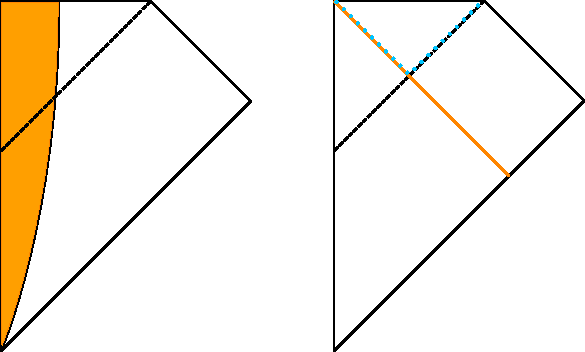
\includegraphics[scale=1]{collapse}
		\end{center}
			\caption{In both diagrams, the upper boundary is the singularity while the left boundary is the origin of the polar coordinates. The other two boundaries are asymptotic to the ones of the Minkowski space. On the left side we have a collapsing cloud of massive particles shown in orange, which forms the black hole. On the right side we have a black hole forming out of an infalling shell of photons, where we have the Schwarzschild geometry above the orange line, and a piece of Minkowski space below it. The event horizon is illustrated as a dashed line, the apparent horizon is shown with blue dots.}\label{collapse}
	\end{figure}	
	Now, how does that lead us to black holes? First of all, real astrophysical black holes are a result of gravitational collapse, like at the end of a star live. But considering massive particles would mean, that we have to include all interactions between them. So for making it convenient, we instead imagine a black hole arise from a spherically symmetric infalling shell of photons. 
	That also leads to the fact, that there is no obstacle while the black hole is formed, like the Schwarzschild radius.
		
	But now the horizon extends into the Minkowski space and we have to make a difference between the \textit{actual horizon} and the \textit{apparent horizon}.
	When you are passing the actual horizon, you will not notice it immediately, even though your fate has already been sealed. This leads to some kind of acausal nature of horizons: Their locations depend on events that have not yet happened. 
	
	For defining the apparent horizon, which will help us, to avoid this acasual nature, we first notice, that the Schwarzschild horizon can be detected locally in time, for any sphere of constant $r$ with $r<1$.\footnote{Here, the Schwarzschild radius is set to $2GM=1$}
	Any null geodesics of these spheres which starts out orthogonal, converges towards other null geodesics of this kind. And if we have a compact 2-dim surface, it is called a \textit{closed trapped surface}.
	
	\textbf{An apparent horizon is now a surface which is a boundary of a connected set of closed trapped surfaces.}
	For to describe the real black hole in one diagram, we take a mixture of Minkowski space and Schwarzschild solution into a Penrose diagram as shown in \textbf{Figure \ref{collapse}.} The apparent horizon is illustrated with blue dots. And as you can see, it does form itself in the same moment when the photon shell crosses the event horizon.
				